\documentclass{article}
\usepackage[utf8]{inputenc}
\usepackage{geometry}
\usepackage{xcolor}
\usepackage{eso-pic}
\usepackage{fancyhdr}
\usepackage{parskip}
\usepackage{microtype}
\usepackage[english]{babel}
\usepackage{url}
\usepackage{amsmath}
\usepackage{amssymb}
\usepackage{amsthm}
\usepackage{longtable}
\usepackage{booktabs}
\usepackage{hyperref}
\usepackage{titlesec}
\usepackage{tikz}
\usetikzlibrary{shapes.geometric, arrows, arrows.meta, positioning, fit, backgrounds, calc}

\definecolor{nato}{HTML}{293757}
\definecolor{footergray}{gray}{0.65}
\definecolor{coreblue}{HTML}{4682B4}
\definecolor{productgreen}{HTML}{228B22}
\definecolor{edupink}{HTML}{DB7093}
\definecolor{visiongold}{HTML}{DAA520}
\definecolor{limitedgray}{HTML}{696969}

\geometry{a4paper,left=3cm,right=3cm,top=3cm,bottom=3cm}
\renewcommand{\familydefault}{\sfdefault}
\setcounter{secnumdepth}{3}

\titleformat{\section}{\color{nato}\Huge\bfseries}{\thesection.}{1em}{}
\titlespacing*{\section}{0pt}{30pt}{12pt}
\titleformat{\subsection}{\color{nato}\LARGE\bfseries}{\thesubsection.}{1em}{}
\titlespacing*{\subsection}{0pt}{20pt}{8pt}
\titleformat{\subsubsection}{\color{nato}\Large\bfseries}{\thesubsubsection.}{1em}{}
\titlespacing*{\subsubsection}{0pt}{10pt}{6pt}

\fancyhf{}
\fancyhead[R]{\small\color{footergray} B-System Technical Note}
\fancyfoot[L]{\small\color{footergray} B-System / BTRON3 Cleanroom}
\fancyfoot[R]{\small\color{footergray}\thepage}
\newcommand\HUGE[1]{\fontsize{40}{40}\selectfont #1}
\renewcommand{\headrulewidth}{0pt}
\renewcommand{\footrulewidth}{0.4pt}
\renewcommand{\footrule}{\color{footergray}\hrule width\textwidth height 0.4pt}

\let\originalfootnotesize\footnotesize
\let\oldverbatim\verbatim
\let\oldendverbatim\endverbatim
\renewenvironment{verbatim}{\originalfootnotesize\oldverbatim}{\oldendverbatim}

\title{B-System: TRON History Lineages}
\author{Synrc Research Center / B-System Project}
\date{September 2026}

\begin{document}

\begin{titlepage}
  \AddToShipoutPictureBG*{\AtPageLowerLeft{\color{nato}\rule{\paperwidth}{\paperheight}}}
  \color{white}\thispagestyle{empty}\vspace*{2.5cm}\centering
  {\Huge \textbf{B-System} \par} \vspace{1.2cm}
  {\HUGE \textbf{BTRON History and Lineages} \par} \vspace{1.5cm}
  {\LARGE \textbf{BTRON1 -- BTRON2 -- BTRON3} \par} \vspace{1.5cm}
  {\large A Historical Analysis of the Three Lineages \par}
  {\large of Japan's Open Architecture Personal Computing Initiative \par} \vspace{1cm}
  {\large Based on TRON Forum Chronology, Personal Media Archives, \par}
  {\large National Diet Library Technical Reports, and Surviving Artifacts \par}
  \vfill
  {\large 2026 \copyright\ Synrc Research Center / B-System Project \par}
\end{titlepage}

\newpage
\maketitle

\begin{abstract}
This B-System technical note provides a rigorous historical and technical examination of the three principal lineages of BTRON (Business TRON), the personal computing subproject of Japan's TRON Project initiated by Ken Sakamura in 1984. Drawing on primary sources including TRON Project Symposium papers, Personal Media product histories, the National Diet Library technical report on PanaCAL ET, and contemporary investigations of surviving ET Master media, it reconstructs the evolutionary paths of BTRON1 (practical 16-bit implementations), BTRON2 (pure TRONCHIP high-end specification), and BTRON3 (microkernel synthesis culminating in B-right/V and Cho-Kanji). Architectural diagrams, chronological tables, and lineage flowcharts illustrate the tension between idealistic pure-TRON designs and pragmatic adaptations to available hardware amid market and geopolitical constraints. The note serves as historical context for the B-System cleanroom reimplementation of BTRON3 Specification 3.20.
\end{abstract}

\tableofcontents
\newpage

\section{Introduction}

The TRON (The Real-time Operating system Nucleus) project, launched in 1984 by Ken Sakamura of the University of Tokyo, represented one of the most ambitious open-architecture computing initiatives of the late twentieth century. Its goal was a vertically integrated ecosystem spanning from embedded microcontrollers to personal workstations and large-scale systems, all designed for a Highly Functionally Distributed System (HFDS) vision of ubiquitous computing. Within this framework, BTRON (Business TRON) was the subproject dedicated to personal computers, workstations, and human-machine interfaces.

BTRON was never a single operating system but a family of specifications evolving in response to hardware realities, market pressures, and project priorities. Three primary lineages emerged:

\begin{itemize}
  \item \textbf{BTRON1} --- the practical 16-bit implementation lineage centred on Intel 80286;
  \item \textbf{BTRON2} --- the pure high-end vision targeting custom TRONCHIP 32-bit processors;
  \item \textbf{BTRON3} --- the pragmatic microkernel synthesis that achieved the most lasting commercial presence through B-right/V and Cho-Kanji (\textit{Ch\=o-Kanji}).
\end{itemize}

These lineages reflect the persistent tension between idealistic pure-TRON designs and the pragmatic necessity of running on available hardware amid intense competition from MS-DOS, the NEC PC-9801 series, and later Microsoft Windows, as well as external pressures including U.S. trade concerns articulated in the 1989 National Trade Estimate Report.

This study examines each lineage in depth, drawing on primary sources such as TRON Project Symposium proceedings, Personal Media documentation, TRON Forum chronology, National Diet Library technical reports, and surviving hardware investigations of the ET Master distribution.

\section{BTRON1}

\subsection{Origins and Specification}

BTRON1 originated as the practical entry point for personal computing within the TRON project. Early roadmaps distinguished a 16-bit BTRON for conventional personal computers, a \(\mu\)BTRON for dedicated word processors, and a higher-end pure-TRON variant planned for the early 1990s. By 1988 the BTRON/286 specification targeted the Intel 80286 and became the foundation of what was formalised as BTRON1 in 1989.

Key design principles included:

\begin{itemize}
  \item the real-body / pseudo-body (\textit{jisshin/kashin}, real/kashi) object model for hypermedia-style data structures;
  \item TAD (TRON Application Databus) as a consistent data-exchange format;
  \item a bitmapped graphical user interface emphasising ease of use and multilingual support, particularly Japanese input;
  \item a focus on educational and business applications.
\end{itemize}

The architecture aimed for consistency across machines while remaining open and royalty-free.

\subsection{Commercial Realisations}

The first major commercial realisation emerged from Matsushita Electric Industrial (later Panasonic) in collaboration with Personal Media. In 1990 the ET Master operating system---a BTRON1 implementation on 80286 hardware---powered the PanaCAL ET educational system. PanaCAL ET featured dedicated audiovisual hardware extensions for multimedia education, LAN connectivity for classroom use, and specialised educational software suites. A 1993 National Diet Library technical report (National Technical Report 39(1), pp.~99--106) details its design as an ``education-oriented computer system''.

Surviving five-disk 3.5-inch 2HD distributions and detailed boot-process investigations confirm its use of protected-mode 80286 features and a distinctive splash screen referencing ``Hypermedia Lab PanaCAL ET''. Contemporary examinations rank ET Master among the earliest commercial BTRON systems and note its sophisticated utilisation of 16-bit protected mode, comparable to contemporary Xenix 286 or OS/2 1.x implementations.

Personal Media continued the lineage with commercial products:

\begin{itemize}
  \item 1B/Note laptop (1991), a Matsushita OEM on Panacom M-series hardware;
  \item 1B/V1 (1994), 1B/V2 (1995), and 1B/V3 (1996) for PC/AT-compatible x86 machines.
\end{itemize}

These retained the BTRON1 core (GUI, text and graphics processing, Japanese input, real/kashi model, TAD) while adapting to more widely available hardware platforms.

\subsection{Chronological Summary of BTRON1 Systems}

\begin{center}
\begin{tabular}{@{}lllc@{}}
\toprule
\textbf{System} & \textbf{Year} & \textbf{CPU} & \textbf{Status} \\
\midrule
BTRON/286 prototype & \(\sim\)1988 & 80286 & Prototype \\
ET Master           & 1990 & 80286 & Commercial \\
1B/Note             & 1991 & 80286-class & Commercial \\
1B/V1               & 1994 & x86 & Commercial \\
1B/V2               & 1995 & x86 & Commercial \\
1B/V3               & 1996 & x86 & Commercial \\
\bottomrule
\end{tabular}
\end{center}

ET Master remains historically distinctive: it was among the earliest commercial BTRON systems, leveraged protected-mode 80286 capabilities at a sophisticated level, and integrated education-specific multimedia hardware. Its survival as a five-disk set and the detailed technical investigations available make it a primary artifact for reconstructing early BTRON1 behaviour.

\subsection{BTRON1 Lineage Diagram}

\begin{center}
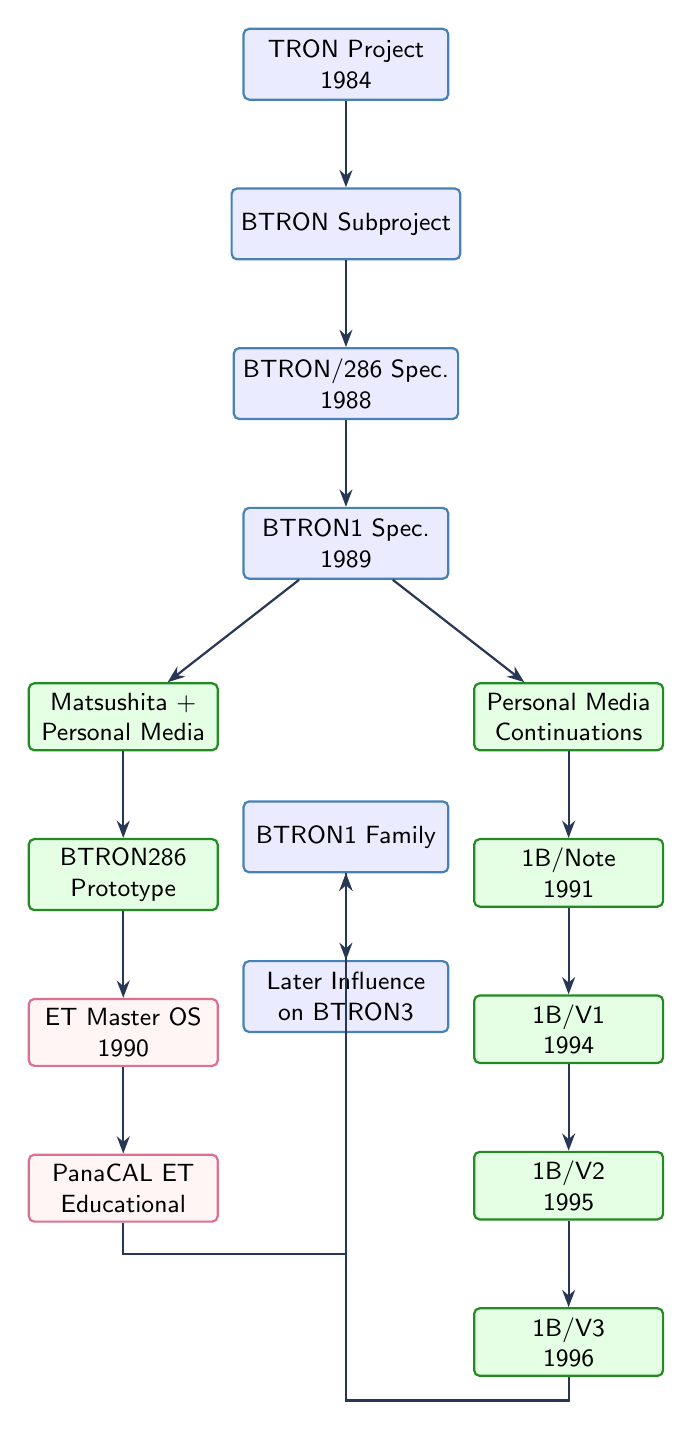
\begin{tikzpicture}[
  node distance=1.1cm and 1.4cm,
  box/.style={rectangle, draw=coreblue, thick, rounded corners=2pt, align=center, fill=blue!8, font=\small, minimum width=2.6cm, minimum height=0.9cm},
  product/.style={rectangle, draw=productgreen, thick, rounded corners=2pt, align=center, fill=green!10, font=\small, minimum width=2.4cm, minimum height=0.85cm},
  edu/.style={rectangle, draw=edupink, thick, rounded corners=2pt, align=center, fill=pink!15, font=\small, minimum width=2.4cm, minimum height=0.85cm},
  arrow/.style={-{Stealth[length=2.2mm]}, thick, color=nato}
]
  \node[box] (tron) {TRON Project\\1984};
  \node[box, below=of tron] (btron) {BTRON Subproject};
  \node[box, below=of btron] (spec286) {BTRON/286 Spec.\\1988};
  \node[box, below=of spec286] (btron1) {BTRON1 Spec.\\1989};

  \node[product, below left=1.3cm and 0.3cm of btron1] (mats) {Matsushita +\\Personal Media};
  \node[product, below right=1.3cm and 0.3cm of btron1] (pm) {Personal Media\\Continuations};

  \node[product, below=of mats] (b286) {BTRON286\\Prototype};
  \node[edu, below=of b286] (et) {ET Master OS\\1990};
  \node[edu, below=of et] (pana) {PanaCAL ET\\Educational};

  \node[product, below=of pm] (note) {1B/Note\\1991};
  \node[product, below=of note] (v1) {1B/V1\\1994};
  \node[product, below=of v1] (v2) {1B/V2\\1995};
  \node[product, below=of v2] (v3) {1B/V3\\1996};

  \node[box, below=2.8cm of btron1] (family) {BTRON1 Family};
  \node[box, below=of family] (later) {Later Influence\\on BTRON3};

  \draw[arrow] (tron) -- (btron);
  \draw[arrow] (btron) -- (spec286);
  \draw[arrow] (spec286) -- (btron1);
  \draw[arrow] (btron1) -- (mats);
  \draw[arrow] (btron1) -- (pm);
  \draw[arrow] (mats) -- (b286);
  \draw[arrow] (b286) -- (et);
  \draw[arrow] (et) -- (pana);
  \draw[arrow] (pm) -- (note);
  \draw[arrow] (note) -- (v1);
  \draw[arrow] (v1) -- (v2);
  \draw[arrow] (v2) -- (v3);
  \draw[arrow] (pana.south) -- ++(0,-0.4) -| (family);
  \draw[arrow] (v3.south) -- ++(0,-0.3) -| (family);
  \draw[arrow] (family) -- (later);
\end{tikzpicture}
\end{center}


\newpage
\section{BTRON2 and TRONCHIP}

\subsection{Specification Focus}

BTRON2 represented the ``pure'' high-end vision of BTRON, targeted at systems built around custom TRONCHIP 32-bit CISC processors rather than commodity x86 hardware. Specification work emphasised a modular hierarchical structure:

\begin{itemize}
  \item an inner kernel as an ITRON2 subset;
  \item an outer kernel;
  \item a shell layer.
\end{itemize}

All operating-system-managed resources---memory, processes, threads---were fully integrated into the real/kashi object model. Additional goals included robust multimedia support and distributed processing capabilities suited to larger-scale workstations.

\subsection{Hardware Target: TRONCHIP}

Hardware targets included evaluation platforms such as Fujitsu's GENESYS equipped with the F32/300 (Gmicro series) and other TRONCHIP variants produced by Fujitsu, Mitsubishi, Hitachi (Gmicro line), Toshiba (TX series), Matsushita (MN10400), and Oki (O32). These complex CISC designs aimed for high performance and architectural consistency with TRON OS specifications but faced severe commercial challenges in cost, power efficiency, and performance relative to evolving x86 processors and emerging RISC alternatives.

\subsection{Implementation and Outcome}

The principal implementation was Personal Media's 2B operating system, detailed in a 1991 TRON Project Symposium paper by N.~Osawa. 2B followed the BTRON2 design philosophy with its three-layer modular hierarchy and was demonstrated on TRON-specification CPUs. Related early pure-TRON workstations such as MCUBE (associated with SIGBTRON) are more closely linked to subsequent BTRON3 developments.

The BTRON2 specification was published around 1992. Limited prototypes existed, but broad commercial productisation never occurred. TRONCHIP viability issues, competition from established PC platforms (especially the NEC PC-9801 series), and shifting project priorities constrained its impact. Practical development consequently moved toward more accessible hardware in the BTRON3 lineage.

\subsection{BTRON2 Lineage Diagram}

\begin{center}
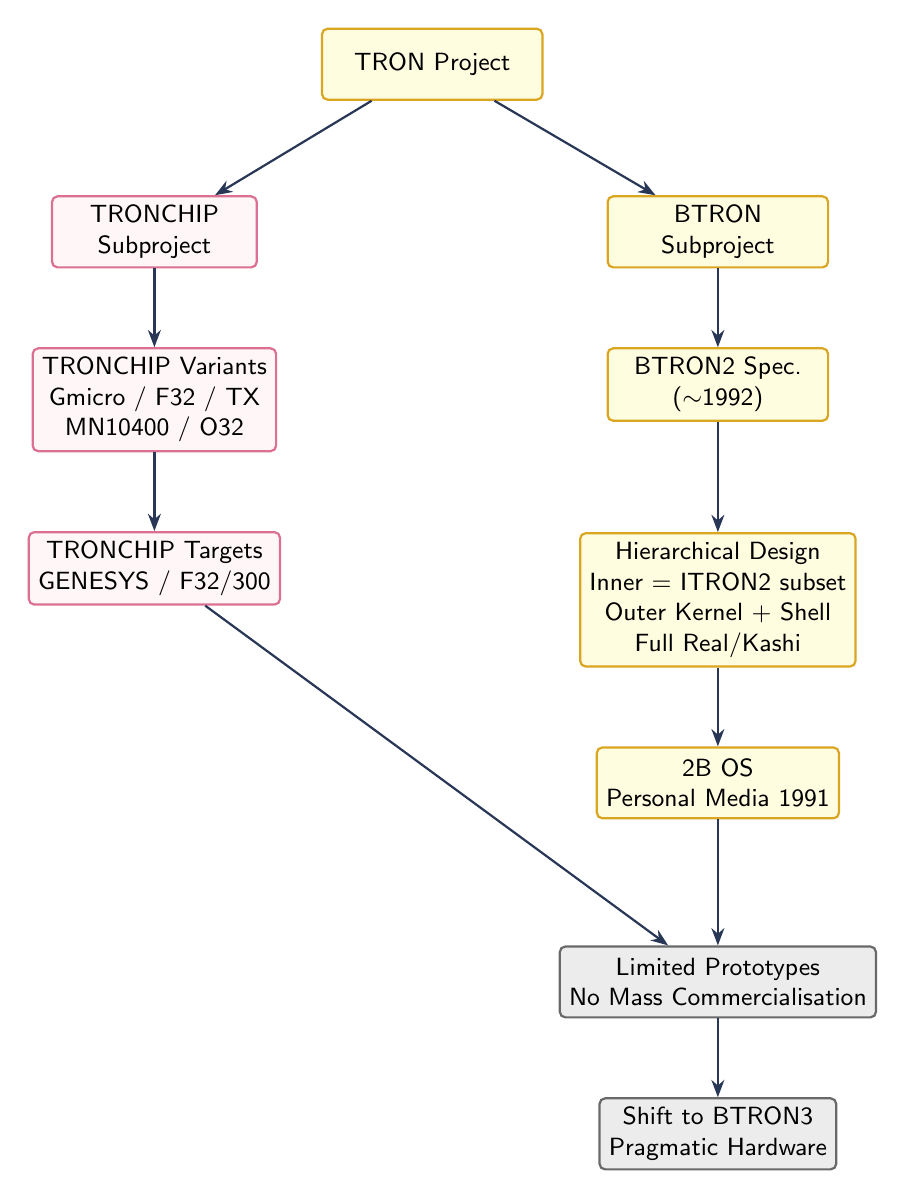
\begin{tikzpicture}[
  node distance=1.0cm and 1.6cm,
  box/.style={rectangle, draw=visiongold, thick, rounded corners=2pt, align=center, fill=yellow!12, font=\small, minimum width=2.8cm, minimum height=0.9cm},
  hard/.style={rectangle, draw=edupink, thick, rounded corners=2pt, align=center, fill=pink!12, font=\small, minimum width=2.6cm, minimum height=0.9cm},
  limited/.style={rectangle, draw=limitedgray, thick, rounded corners=2pt, align=center, fill=gray!15, font=\small, minimum width=2.6cm, minimum height=0.9cm},
  arrow/.style={-{Stealth[length=2.2mm]}, thick, color=nato}
]
  \node[box] (tron) {TRON Project};
  \node[hard, below left=1.2cm and 0.8cm of tron] (chip) {TRONCHIP\\Subproject};
  \node[box, below right=1.2cm and 0.8cm of tron] (btron) {BTRON\\Subproject};

  \node[hard, below=of chip] (variants) {TRONCHIP Variants\\Gmicro / F32 / TX\\MN10400 / O32};
  \node[box, below=of btron] (btron2) {BTRON2 Spec.\\(\(\sim\)1992)};

  \node[box, below=1.4cm of btron2] (design) {Hierarchical Design\\Inner = ITRON2 subset\\Outer Kernel + Shell\\Full Real/Kashi};
  \node[box, below=of design] (impl) {2B OS\\Personal Media 1991};
  \node[hard, below=of variants] (target) {TRONCHIP Targets\\GENESYS / F32/300};

  \node[limited, below=1.6cm of impl] (outcome) {Limited Prototypes\\No Mass Commercialisation};
  \node[limited, below=of outcome] (shift) {Shift to BTRON3\\Pragmatic Hardware};

  \draw[arrow] (tron) -- (chip);
  \draw[arrow] (tron) -- (btron);
  \draw[arrow] (chip) -- (variants);
  \draw[arrow] (btron) -- (btron2);
  \draw[arrow] (btron2) -- (design);
  \draw[arrow] (design) -- (impl);
  \draw[arrow] (variants) -- (target);
  \draw[arrow] (impl) -- (outcome);
  \draw[arrow] (target) -- (outcome);
  \draw[arrow] (outcome) -- (shift);
\end{tikzpicture}
\end{center}

In essence, the BTRON2 lineage was primarily a specification-and-prototype branch embodying the high-end, silicon-to-OS pure-TRON ideal. It remained specialised and experimental.

\newpage
\section{BTRON3}

\subsection{Architectural Synthesis}

BTRON3 synthesised ideas from both prior lineages while adopting a more pragmatic architecture. Personal Media formulated the BTRON3 specification on BTRON1 foundations, incorporating a \(\mu\)ITRON-derived microkernel (initially based on the University of Tokyo's ItIs Phase~3, later evolved to I-right). This enabled 32-bit operation, improved modularity, and support for loosely coupled distributed environments.

\subsection{Key Implementations}

Key implementations began with 3B on pure-TRON hardware such as the MCUBE workstation (Fujitsu Gmicro F32/300). Practical commercial success arrived with:

\begin{itemize}
  \item B-right (micro-BTRON adaptations for PDAs, exemplified by the 1996 BrainPad TiPO on NEC V810);
  \item B-right/V for PC/AT-compatible machines (released 1998).
\end{itemize}

From B-right/V R2 (1999) onward the product was marketed as Cho-Kanji (\textit{Ch\=o-Kanji} / Super Kanji), emphasising extensive multilingual and multi-character-set support via TRON Code. TRON Code planes supported tens to hundreds of thousands of characters, including rare historical forms, Braille, and CJK variants that exceeded early Unicode coverage in certain domains for more than a decade.

\subsection{Enduring Features and Continuity}

Cho-Kanji retained core BTRON strengths---the real/kashi hypermedia model, TAD, consistent GUI, and efficient resource utilisation---while running on commodity x86 hardware (later via VMware Player for modern systems). Subsequent releases (Cho-Kanji~2 through Cho-Kanji~V, up to R4.560 in recent years) added larger character sets (GT Typeface / GT Mincho), improved storage support, and continued refinement. Related middleware such as T-Shell on T-Kernel extended concepts into the later T-Engine project.

\newpage
\subsection{BTRON3 Lineage Diagram}

\begin{center}
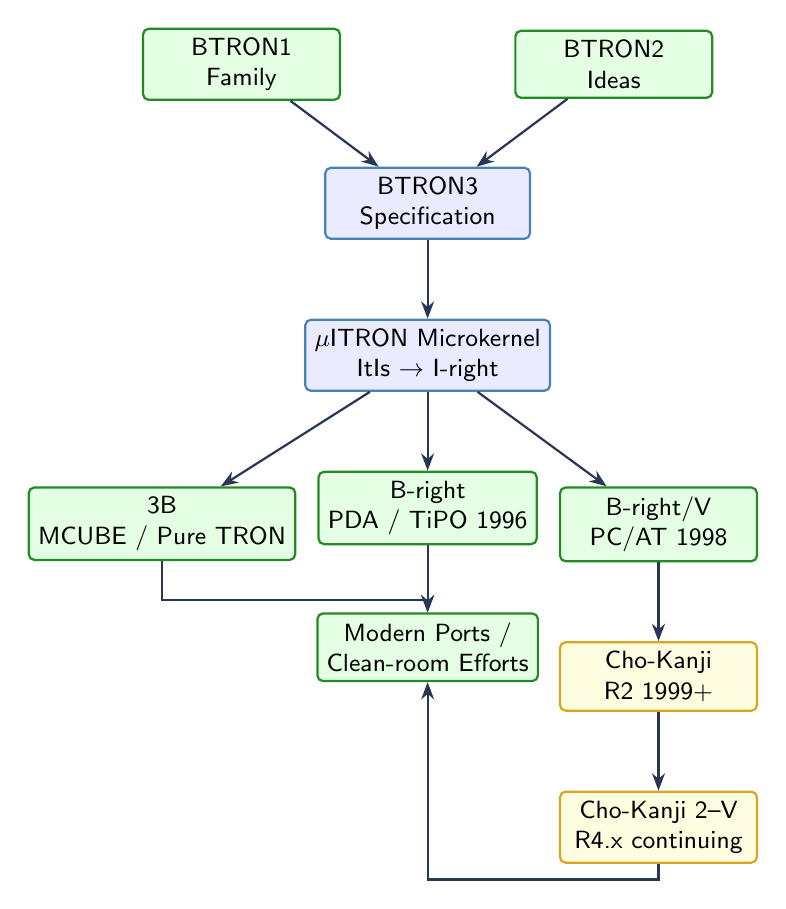
\begin{tikzpicture}[
  node distance=1.0cm and 1.3cm,
  box/.style={rectangle, draw=productgreen, thick, rounded corners=2pt, align=center, fill=green!10, font=\small, minimum width=2.5cm, minimum height=0.85cm},
  synth/.style={rectangle, draw=coreblue, thick, rounded corners=2pt, align=center, fill=blue!8, font=\small, minimum width=2.6cm, minimum height=0.9cm},
  multi/.style={rectangle, draw=visiongold, thick, rounded corners=2pt, align=center, fill=yellow!12, font=\small, minimum width=2.5cm, minimum height=0.85cm},
  arrow/.style={-{Stealth[length=2.2mm]}, thick, color=nato}
]
  \node[box] (b1) {BTRON1\\Family};
  \node[box, right=2.2cm of b1] (b2) {BTRON2\\Ideas};
  \node[synth, below=1.3cm of $(b1)!0.5!(b2)$] (spec) {BTRON3\\Specification};

  \node[synth, below=of spec] (micro) {\(\mu\)ITRON Microkernel\\ItIs \(\rightarrow\) I-right};

  \node[box, below left=1.2cm and 0.1cm of micro] (threeb) {3B\\MCUBE / Pure TRON};
  \node[box, below=of micro] (bright) {B-right\\PDA / TiPO 1996};
  \node[box, below right=1.2cm and 0.1cm of micro] (brightv) {B-right/V\\PC/AT 1998};

  \node[multi, below=of brightv] (cho) {Cho-Kanji\\R2 1999+};
  \node[multi, below=of cho] (later) {Cho-Kanji 2--V\\R4.x continuing};

  \node[box, below=2.8cm of micro] (modern) {Modern Ports /\\Clean-room Efforts};

  \draw[arrow] (b1) -- (spec);
  \draw[arrow] (b2) -- (spec);
  \draw[arrow] (spec) -- (micro);
  \draw[arrow] (micro) -- (threeb);
  \draw[arrow] (micro) -- (bright);
  \draw[arrow] (micro) -- (brightv);
  \draw[arrow] (brightv) -- (cho);
  \draw[arrow] (cho) -- (later);
  \draw[arrow] (threeb.south) -- ++(0,-0.5) -| (modern);
  \draw[arrow] (bright.south) -- ++(0,-0.3) -| (modern);
  \draw[arrow] (later.south) -- ++(0,-0.2) -| (modern);
\end{tikzpicture}
\end{center}

BTRON3 achieved the greatest practical continuity. While never challenging Windows or Linux for mainstream dominance, Cho-Kanji remains available and continues to serve niche users who value its character handling, hypermedia model, and efficient design. Recent clean-room efforts (for example, B-System implementations of BTRON3 specification 3.20) demonstrate ongoing interest in preserving and modernising the architecture.

\section{Conclusion}

The three lineages of BTRON illustrate the evolution of an idealistic open architecture under real-world constraints. BTRON1 delivered the first commercial systems and educational experiments (ET Master / PanaCAL ET and the 1B series). BTRON2 embodied the pure high-end TRONCHIP vision that remained largely experimental. BTRON3 pragmatically combined prior ideas with a microkernel approach, producing the longest-lived products in B-right/V and Cho-Kanji.

External factors---U.S.\ trade scrutiny in 1989 that discouraged mandatory school adoption, the commercial difficulties of custom CISC TRONCHIPs, and the rapid rise of Windows---limited broader impact. Yet the project's open specifications, emphasis on consistent human-machine interfaces and data models, multilingual capabilities, and the real/kashi hypermedia concepts left a distinctive legacy. The parallel success of ITRON in embedded systems further validates the broader TRON approach.

Today, surviving documentation, hardware artifacts, and modern reimplementations ensure that the intellectual contributions of BTRON's three lineages remain accessible for historical study and potential future inspiration in open, human-centred computing architectures.

\vspace{1.5cm}
\begin{center}
\textit{Primary sources consulted include TRON Forum chronology, Personal Media BTRON product histories,}\\
\textit{TRONWARE Vol.~7, National Diet Library technical reports on PanaCAL ET,}\\
\textit{TRON Project Symposium proceedings (especially 1991 papers on 2B),}\\
\textit{and contemporary technical investigations of surviving ET Master media.}
\end{center}

\end{document}
